\chapter{Background}

This chapter aims to provide an overview on the fundamentals of Space Flight Dynamics that constitute the theoretical basis of this thesis, with a specific focus on Earth Observation applications in Low Earth Orbit (LEO), as well as a literature review on orbit management methods addressed by this work.

\section{Space Flight Dynamics Overview}

Orbital Mechanics, Astrodynamics, Astronautics and Space Flight Dynamics are all titles of university courses whose principal topic is two-body orbital motion, that involves orbit determination, orbital flight time, and orbital maneuvers \cite{kluever2018space}.
In this context, a proper definition of the subject can be the following: the study of the motion of man-made objects in space, subject to both natural and artificially induced forces \cite{griffin2004space}.

\subsection{Satellite State Representations}

% There are a number of independent parameters describing the size, shape, and spatial position of an orbit.
% Six of these have become the parameters of choice to define and describe an orbit.
To define the \textit{state} of a satellite in space six quantities are required, and they may take on many equivalent forms.
Whatever the form, the collection is called either a \textit{state vector}, usually associated with position and velocity vectors, or an \textit{element set}, typically used with scalar magnitude and angular representations of the orbit called \textit{orbital elements}.
Either set of quantities completely specify the two-body orbit and provide a complete set of initial conditions for solving an initial value problem class of differential equations.
Time is always associated with a state vector and is often considered a seventh component.
State vectors and element sets are referenced to a particular coordinate frame \cite{vallado2013fundamentals}.

This thesis will use both state vectors and a specific element set.
The latter, which is also the most common one in this field, is represented by the \textit{\textbf{classical orbital elements}}:
\begin{itemize}
    \item Semimajor axis, \textit{a}: the orbit size is defined by one half of the major axis dimension
    \item Eccentricity, \textit{e}: the ratio of minor to major dimensions of an orbit defines the shape
    \item Inclination, \textit{i}: the angle between the orbit plane and the reference plane or the angle between the normals to the two planes
    \item Longitude of the ascending node or Right Ascension of the Ascending Node (RAAN), $\Omega$: the angle between the vernal equinox vector and the ascending node measured in the reference plane in a couterclockwise direction as viewed from the northern hemisphere
    \item Argument of periapsis, $\omega$: the angle from the ascending node to the periapsis, measured in the orbital plane in the direction of spacecraft motion. The ascending node is the point where the spacecraft crosses the reference plane headed from south to north. the line of nodes is the line formed by the intersection of the orbit plane and the reference plane
    \item True anomaly, $\nu$: the sixth element locates the spacecraft position on the orbit
\end{itemize}
\cite{brown1998spacecraft}
%---------IMMAGINI---------

This thesis work makes also use of the \textit{argument of latitude, u}, which is the angle measured between the ascending node and the satellite's position vector in the direction of satellite motion.
A relation that is always valid exists between classical orbital elements and the argument of latitude \cite{vallado2013fundamentals}:
\begin{equation} \label{eq:argl}
    u = \omega + \nu
\end{equation}
One more element that is often used is the \textit{mean anomaly, M}, which is the angle between the periapsis of an orbit and the position of an imaginary body that orbits in the same period as the real one but at a constant angular speed (circular orbit).
The angular speed assigned to the imaginary body is the satellite's average angular velocity over one orbit, and is called \textit{mean motion, n} \cite{ridpath2012dictionary}.

This research utilizes also another element set which results necessary to address case studies of past missions: the \textit{Two-line element set} (TLE).
A two-line element consists of a satellite identifier, an epoch, six orbital elements and a \textit{B*} term related to the ballistic coefficient \cite{riesing2015orbit}.
These elsets are available to the general public through Air Force Space Command (AFSPC) \cite{vallado2013fundamentals}.

The elements of a TLE are shown in equation \ref{eq:tle} \cite{vallado2013fundamentals}, where:
\begin{itemize}
    \item[-] the bars on  the mean motion and semimajor axis denote \textit{Kozai mean values} 
    \item[-] the numerators of the first two elements of the second line represent mean motion rate and acceleration
    \item[-] $\frac{c_D A}{m}$ corresponds to the inverse of the \textit{ballistic coefficient, BC}
    \item[-] $\rho_0$ is the atmospheric density at perigee of the orbit
    \item[-] $R_\mathTerra$ defines an Earth Radius of 6378.135 km
    \item[-] the epoch is expressed in Coordinate Universal Time (UTC)
\end{itemize}

\begin{equation} \label{eq:tle}
    \begin{split}
        \bar{n}=\sqrt{\frac{\mu}{\bar{a}^{3}}} \;\;\;\;\;\;\;\;\;\; e \;\;\;\;\;\;\;\;\;\; i \;\;\;\;\;\;\;\;\;\; \Omega \;\;\;\;\;\;\;\;\;\; \omega \;\;\;\;\;\;\;\;\;\; M \\
        \frac{\dot{n}}{2} \;\;\;\;\;\;\;\;\;\;\;\; \frac{\ddot{n}}{6} \;\;\;\;\;\;\;\;\;\;\;\; B^* = \frac{1}{2} \frac{c_D A}{m} \rho_0 R_\mathTerra \;\;\;\;\;\;\;\;\;\;\;\; UTC
    \end{split}
\end{equation}

\subsection{Reference Frames}
Two types of reference frames are adopted by this research: the geocentric-inertial coordinate system and the geographic-body-fixed system.
The origin of both systems is the center of mass of the central body, which in all case studies of this work is the Earth.
They will therefore be labeled Earth-centered inertial (ECI) and Eart-centered Earth-fixed (ECEF) coordinate frames, respectively.

\subsubsection{Earth-centered inertial}
The ECI system is shown in FIGURE???.
The equatorial plane is the reference plane.
The X axis is the vernal equinox vector, and the Z axis is the spin axis of the Earth; north is positive.
The axes are fixed in inertial space or fixed with respect to the stars \cite{brown1998spacecraft}.

\subsubsection{Earth-centered Earth-fixed}
FIGURE shows a representation of the ECEF reference frame.
The system is Earth-centered and fixed to the rotating Earth \cite{vallado2013fundamentals}.
Considering the ECI, the Z axis is the same, while the X axis always points towards the Greenwich meridian.
Satellite ground track is commonly plotted in this coordinate system \cite{brown1998spacecraft}.

\subsection{Orbital Perturbations} \label{perturbations}
Orbital perturbations are deviations from a normal, idealized, or undisturbed motion.
Introducing an alteration from two-body problem assumptions, the actual motion will vary due to perturbations caused by other bodies, and additional forces not considered in Keplerian motion \cite{vallado2013fundamentals}.
This subsection provides an overview of the main perturbations for an Earth orbiting spacecraft.

\subsubsection{Earth's Gravity Field}
Spinning celestial bodies are nor perfect spheres, but they are much more similar to oblate spheroids.
For such a planet, the spin axis can be considered as the axis of rotational symmetry and the gravitational field will vary with the latitude as well as radius.
The planet's oblateness provides a rotationally symmetric perturbation $\Phi$, which does not depend on the longitude \cite{curtis2020orbital}.

In particular, $\Phi$ is given by an infinite series characterized by the so-called \textit{zonal harmonics} $J_k$ of the planet of reference.
Considering a spherical coordinate system for convenience, with origin at the planet's center of mass and third axis as the axis of rotational symmetry,
in this series, shown in equation \ref{eq:harmonics_series}, $r$ and $\phi$ are the distance from the origin and the polar angle respectively, $\mu$ is the Earth's standard gravitational parameter, $R$ the equatorial radius and $P_k$ represent the Legendre polynomials \cite{curtis2020orbital}.
\begin{equation} \label{eq:harmonics_series}
    \Phi (r,\phi) = \frac{\mu}{r} \sum_{k=2}^{\infty} J_k \left(\frac{R}{r} \right)^k P_k (\cos{\phi})
\end{equation}
The zonal harmonics are non-dimensional quantities which are evaluated from satellite observation mission around the planet.
The summation starts from $k = 2$, and the Earth's set of zonal harmonics is highly dominated by $J_2$.
Taking into account only $J_2$ and starting from equation \ref{eq:harmonics_series}, it is possible to derivate the perturbing gravitational acceleration due to the respective zonal harmonic \cite{curtis2020orbital}:
\begin{equation} \label{eq:j2_acc}
    \vec{a}_{J_2} = \frac{3}{2} \frac{J_2 \mu R^2}{r^4} \left[\frac{x}{r}\left(5 \frac{z^2}{r^2} - 1 \right)\hat{\textbf{i}} + \frac{y}{r}\left(5 \frac{z^2}{r^2} - 1\right)\hat{\textbf{j}} + \frac{z}{r}\left(5 \frac{z^2}{r^2} - 3\right)\hat{\textbf{k}} \right]
\end{equation}

The right ascension $\Omega$ and the argument of perigee $\omega$ are significantly affected by oblateness \cite{curtis2020orbital}.
% Their variation in time is described by equations \ref{eq:5} and \ref{eq:6} respectively \cite{curtis2020orbital}:
% \begin{equation} \label{eq:5}
%     \dot{\Omega} = - \left[\frac{3}{2} \frac{\sqrt{\mu} J_2 R^2}{(1-e^2)^2 a^{7/2}}\right]\cos{i}
% \end{equation}
% \begin{equation} \label{eq:6}
%     \dot{\omega} = - \left[\frac{3}{2} \frac{\sqrt{\mu} J_2 R^2}{(1-e^2)^2 a^{7/2}}\right] \left(\frac{5}{2} \sin^2{i} - 2\right)
% \end{equation}

It is necessary to underline that the Earth's gravitational field vary not only with latitude but also with longitude due to irregularities in geometry and mass distribution \cite{curtis2020orbital}.
However, with negligible approximation, it is definitely reasonable to consider only oblateness with $J_2$ effects in LEO missions, which is the major force for this range of altitudes, second only to Earth's gravity \cite{brown1998spacecraft}.
In light of the above, this thesis will take into account only $J_2$ forces with respect to the Earth's gravity field perturbations.

\subsubsection{Atmospheric Drag}
The residual atmosphere present at a few hundred kilometers of altitude strongly influences the motion of satellites in LEO.
The basic equation of the perturbing specific force (force per unit mass) due to drag is the following \cite{vallado2013fundamentals}:
\begin{equation} \label{eq:drag_acc}
    \vec{a}_{drag} = - \frac{1}{2} \frac{C_D A}{m} \rho V_{rel}^{2} \frac{\vec{V_{rel}}}{|\vec{V_{rel}}|}
\end{equation}
In equation \ref{eq:drag_acc}, $\frac{m}{C_D A}$ is again the ballistic coefficient, that already appeared in the TLE representation (equation \ref{eq:tle}):
$m$ is the mass of the spacecraft, $A$ represents the cross-sectional area of the satellite with respect to the atmosphere and $C_D$ is the drag coefficient, a dimensionless parameter which takes into account every aerodynamic configuration aspect of the body with respect to the drag forces \cite{sadraey2009drag}.
The value of the drag coefficient for satellites in the upper atmosphere is generally around 2.2 \cite{vallado2013fundamentals};
this number has been considered for all the case studies of the thesis.
Finally, the velocity vector $\vec{V_{rel}}$ is relative to the atmosphere, as well as the cross section.

The main effects provided by aerodynamic drag are changes in the semimajor axis and eccentricity of the orbit and an accurate description of the atmospheric properties is crucial for the evaluation of drag on satellites \cite{vallado2013fundamentals}.
However, uncertainties in the time variance of upper atmosphere make perfect prediction of spacecraft drag impossible \cite{brown1998spacecraft}.
More in depth, the density changes because of a complex interaction between three factors: the nature of the atmosphere's molecular structure, the incident solar flux, and geomagnetic interactions.
Several atmospheric models can be found in literature, either static or time-varying.
The static ones are less accurate, but definitely simpler than the time-varying models, thanks to the assumption of all constant parameters \cite{vallado2013fundamentals}.
This thesis exploits three different models, depending on the applications addressed in the case studies.

The first model considered by this research is static: the exponential model, valid in the range of altitudes between 0 and 1000 km.
It assumes a spherically symmetrical distribution of particles of the atmosphere, in which the density decreases exponentially with increasing the altitude according to equation \ref{eq:exp_model} \cite{vallado2013fundamentals}
\begin{equation} \label{eq:exp_model}
    \rho = \rho_0 \exp{\left[- \frac{h - h_0}{H}\right]}
\end{equation}
where $\rho_0$ and $h_0$ represent a reference density and altitude respectively and $H$ is the scale height.

The second atmospheric model, still static, is the Standard Atmosphere published in 1976 by the U.S. Committee on Extension to the Standard Atmosphere (COESA), valid drom 0 to 1000 km of altitude.
It is an ideal, steady-state model of the Earth's atmosphere at a latitude of $45^{\circ}$N in moderate solar activity conditions \cite{vallado2013fundamentals}.

Finally, Jacchia-Bowman 2008 (JB2008) is an empirical time-varying atmospheric density model. It revises and improves the earlier Jacchia-Bowman 2006 which is based on the diffusion equations of the Jacchia 71 model.
JB2008 takes into account factors like solar irradiances, computed from driving solar indices based on orbit-based sensor data.
Density variations are described by semiannual density equations based on 81-day average solar indices, as well as from temperature equations that include corrections for diurnal and latitudinal effects.
Geomagnetic effects are modeled too.
The model is validated in the altitude range of 175 to 1000 km through comparisons with accurate daily density drag data previously collected for numerous satellites, existing atmospheric models and other measurements from several Earth orbiting satellite missions \cite{bowman2008jb2006,bowman2008new}.

\subsubsection{Third-Body Perturbations}
All the orbital elements are periodically affected by the gravitational forces of the Sun and the Moon.
Similarly to what is triggered by the Earth's equatorial bulge, they apply an external torque to the orbits and cause the angular momentum to rotate.
This perturbation is highly negligible in LEO, where the main effects are provided by $J_2$ and aerodynamic drag \cite{wertz2009orbit}.
However, low Earth orbits characterized by a constant geometry with respect to the perturbing body can be affected by emphasized long-period effects.
This is the case of Sun-synchronous orbits (SSO), for which the constant pattern with the Sun causes a long-term phenomenon of variation of the inclination (around 0.05 degrees per year) \cite{giacaglia1994long}.
Although this number might appear meaningless, inclination is critical to SSO, as will be explained in paragraph \ref{sso_paragraph}.

\subsubsection{Solar-Radiation Pressure}
The last perturbation treated by this thesis is the solar-radiation pressure (SRP), which induces periodic variations in all the orbital elements.
SRP generally becomes significant above 800 km of altitude, as drag becomes less important. Below this threshold, it might be neglected \cite{wertz2009orbit}.
The perturbing acceleration can be approximated by the following equation \cite{vallado2013fundamentals}
\begin{equation} \label{eq:srp_acc}
    \vec{a}_{SRP} = - \frac{p_{SRP} c_{R} A_{\mathSun}}{m_{sat}} \frac{\vec{r}_{\mathTerra \mathSun}}{|\vec{r}_{\mathTerra \mathSun}|}
\end{equation}
$p_{SRP}$ is the solar pressure, which is a quantity representing the change in momentum per unit area, derived by the ratio between the solar flux and the speed of light.
The reflectivity, $c_R$, a value between 0.0 and 2.0, models the type of interaction between radiation and surface exposed to the Sun, $A_{\mathSun}$ \cite{vallado2013fundamentals}.
$m_{sat}$ is trivially the mass of the satellite.

\subsection{Mean Orbital Elements}
The previous subsection has described how orbital perturbations generate continuous variations and oscillations in the orbit elements.
The values of the elements at a single point in time, which are periodically and secularly affected by the perturbing forces, are called \textit{osculating elements}.
On the other side, it is possible to define the \textit{mean orbit elements}, which represent the average motion over a span of time \cite{wertz2009orbit}.
In this way it is possible to obtain a representation of the orbital motion removing short and long-periodic effects induced by perturbations.
And for most operational purposes, conversion from osculating to mean elements is indispensable \cite{walter1967conversion}.
Indeed, applications addressed by this work, like station-keeping and differential drag, require the secular behavior of the satellite to be implemented.

The oblateness of the Earth is the main guilty of periodic effects, provoking variations in all osculating elements, as well as all the other zonal harmonics.
On the other hand, only even zonal gravitational harmonics and atmospheric drag give raise to secular effects in osculating elements, which are constant or non-periodic.
Aerodynamic drag secular perturbation plays a crucial role in LEO \cite{der1996conversion}.

Figure \ref{osc_vs_mean_sma} shows the comparison between osculating and mean semi-major axis of a LEO satellite motion over the course of four months.
The orbital decay induced by the atmospheric drag secular effect is evident, as well as the periodic consequences of $J_2$ perturbation.
\begin{figure}[h] 
    \begin{center}
        \textbf{Semi-Major Axis}\par\medskip
        %\import{img}{osc_vs_mean.pgf}
    \end{center}
    \caption{Osculating vs. mean semi-major axis for a LEO satellite under atmospheric drag and $J_2$ perturbations.}
    \label{osc_vs_mean_sma}
\end{figure}

Several perturbation techniques have been proposed to perform the conversion between osculating and mean elements. 
Brouwer and Kozai works were ones of the first methods appeared in literature, both consisting of first order solutions which take into account the Earth's asphericity but neglect drag effects \cite{arnas2022analytic}.
This thesis uses a refinement of Brouwer's approach, suggested by Lyddane, which solves zero eccentricity and inclination singularities that are involved in the original theory.
Moreover, the algorithm will account only first order $J_2$ terms \cite{schaub2002analytical}.

\section{Specialized Orbits}
\textit{Specialized orbits} are the results of specific orbital features selected during the design of a mission, which can be simply related to the orbit period or, more commonly, to one of the main orbit perturbations \cite{wertz2009orbit}. 
In this section, two special Earth orbits will be analysed, both of interest for the purposes of the thesis.

\subsection{Sun-Synchronous Orbit} \label{sso_paragraph}
Sun-synchronous orbits are specialized orbits characterized by a constant geometry with the Sun over time \cite{vallado2013fundamentals}. 
They are used for several reasons, from technical needs like that ones deriving from thermal and electric power subsystems of the spacecraft to application requirements such as remote sensing.
Indeed, a constant Sun angle is very precious for missions working with electro-optical sensors \cite{brown1998spacecraft}.
This is the case, for instance, of hyperspectral technology. 

An SSO can be obtained by matching the Westward motion of the line of nodes (\textit{regression of the nodes}) to the solar motion projected on the equator, like shown in equation \ref{sso_raan} \cite{brown1998spacecraft}.
\begin{equation} \label{sso_raan}
    \dot{\Omega} = 360^{\circ} / 365.242\;days = 0.9856\;^{\circ}/day 
\end{equation}
This will allow the satellite's line of nodes to keep a constant angular separation with respect to the Sun.
This separation can be achieved with very good approximation only considering the dominant cause of the secular motion of RAAN: $J_2$ perturbation.  
The secular behavior of $\Omega$ induced by the oblateness is function of semi-major axis, eccentricity and inclination and is given by the following formula \cite{vallado2013fundamentals}:
\begin{equation} \label{raan_variation}
    \dot{\Omega}(a,e,i) = - \frac{3n R_{\mathTerra}^2 J_2}{2a^2 (1-e^2)^2} \cos{i}
\end{equation}
Equations \ref{sso_raan} and \ref{raan_variation} suggest that to achieve the proper $\dot{\Omega}$ of an SSO, the inclination has to be more than 90$^\circ$ (\textit{retrograde orbit}), so that the term $\cos{i}$ will become negative \cite{wertz2009orbit}.
As for the other two variables, eccentricity is generally supposed to be near-zero because low-Earth orbits usually imply very small values of $e$.
Hence, with the assumption of $e=0$, an SSO will be characterized by a direct relationship between $a$ and $i$.
Figure \ref{inc_h_sso} shows the range of inclinations and altitudes that would provide the proper regression of nodes.
\begin{figure} 
    \begin{center} 
        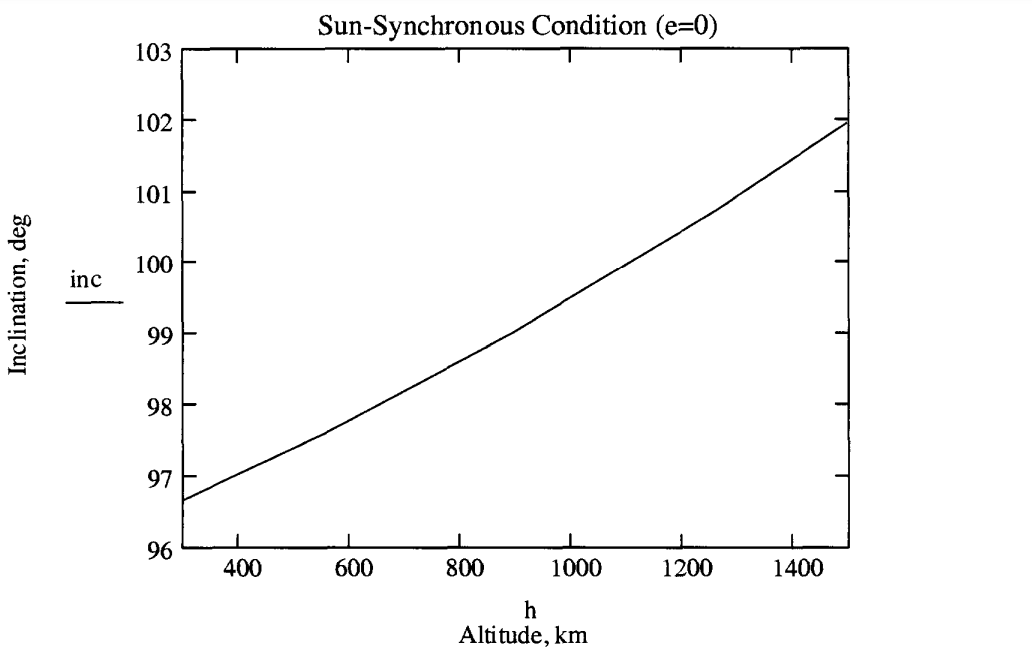
\includegraphics[scale=0.5]{img/inc_vs_h_sso.png}
    \end{center}
        \caption{SSO condition: inclination vs. altitude ($e=0$) \cite{brown1998spacecraft}.}
        \label{inc_h_sso}
\end{figure}

In addition, it is possible to select the initial value of the RAAN between 0 and 360 degrees according to the mission requirements for example \cite{vallado2013fundamentals}.
The angle between the ascending node and the direction of the Sun is commonly labeled like \textit{Mean Local Time of the Ascending Node} (MLTAN), because of the relative time to the noon meridian.
This is a crucial design parameter because, while for an arbitrary orbit the MLTAN would continually change, for a Sun-synchronous orbit it will remain constant \cite{boain2004ab} (not only at the nodes, but at any latitude).

In order to provide a better understanding of the concepts, figure \ref{sso_curtis} shows an example of an SSO with an LTAN of 15:00.
\begin{figure} 
    \begin{center} 
        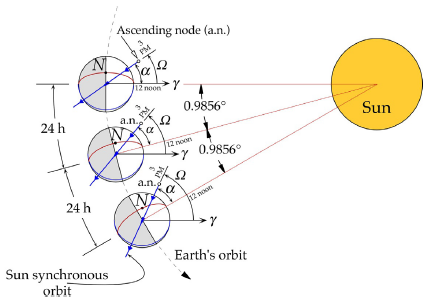
\includegraphics[scale=1]{img/sso_curtis.png}
    \end{center}
        \caption{Sun-synchronous orbit 15:00 LTAN illustration \cite{curtis2020orbital}.}
        \label{sso_curtis}
\end{figure}

\subsection{Repeat-Groundtrack Orbit} \label{repeat_groundtrack}
The peculiarity of a \textit{repeat-groundtrak orbit} is the repetitive transit of the satellite to the same location relative to the surface of the Earth after a certain time interval \cite{wertz2009orbit}.
Hence, they are used by missions which need to periodically revisit a specific point on the Earth \cite{vallado2013fundamentals}, playing an interesting role in remote sensing applications.

Considering $j$ orbit periods and the relative $k$ days spent, an orbit is repetitive if and only if the ratio $Q$ between $j$ and $k$ is a rational number, where $Q$ represents the number of orbits per day.
This means that $j$ and $k$ are integer and prime to each other.
For instance, if a satellite performs 15.25 orbits per day, it will make a 4-day repeating ground track, because the respective rational $Q$ is given by $j=61$ orbits in $k=4$ days \cite{wertz2009orbit}.
$k$ is typically known as the \textit{revisit time} of the spacecraft, defined as the time elapsed between two successive observations of the same ground point \cite{luo2017novel}.
It is necessary to underline that the effects of perturbations should be taken into account in order to obtain accurate repetition properties, since the actual period appears more complex \cite{wertz2009orbit}. 

In light of the above, it can be easily understood that the minimum achievable revisit time for a generic orbit is 1 day.
However, mission objectives might require shorter revisit times.
The solution to this issue is the design of a constellation of satellites, as will be discussed later.



\section{Satellite Constellations}
\subsection{Walker Delta Constellation}
\subsection{Constellation Design}

\section{Orbit Maintenance}
Over the life of a space mission, the need to adjust or maintain the orbit elements might arise. In general, orbit maintenance is required because of two main reasons:
 targeting to reach an end orbit or position (such as a rendezvous maneuver), or to maintain absolute or relative orientations (as for station-keeping) \cite{wertz2009orbit}.

This thesis studies two different scenarios of orbit management. The first one is the \textit{station-keeping}, which aims at periodically restoring the mission nominal altitude. 
Secondly, the study of the \textit{orbit phasing} is carried out with the purpose of achieving the desired pattern of a group of satellites along the same orbit.

\subsection{Station-Keeping}
From LEO to geostationary orbit (GEO), station-keeping maneuvers must be considered due to perturbations, if requested by one or more mission requirements.  
In the case of Earth observation applications, electro-optical sensors and radars are generally designed to work approximately at a specific distance from the ground. 
In addition, the repetition factor $Q$ introduced in the paragraph \ref{repeat_groundtrack} will be significantly altered by even small changes in the semimajor axis.
The maneuver of station-keeping that counteracts the orbital decay in LEO is called \textit{drag makeup maneuver}. 
Assuming that this distance has been reached from the satellite, in LEO it will be threatened over time by atmospheric drag secular effects.

\subsubsection{Edelbaum-Kechichian Theory}
An analytic solution for the optimum low-thrust transfer between inclined circular orbits of different radius is provided by the equations of \textit{Edelbaum} reformulated by \textit{Kechichian} in 1992 \cite{edelbaum1961propulsion, kechichian1992reformulation}.
This thesis takes advantage of this theory to compute $\Delta V$, burning time and related acceleration needed to satisfy the requirements of station-keeping.

The problem obviously needs the thrust force acceleration $f$ as input parameter, deriving from the ratio between the thrust provided by the thruster and the spacecraft mass, is broken down into three mutually orthogonal components:
the first one is tangential to the velocity vector of the satellite, the second component is normal to the orbital plane, and the last one is normal to the other two.
They are expressed in terms of two angles: 
$\alpha$ is the angle between the velocity vector and the component of the thrust vector in the plane of the orbit,
while $\beta$ represents the angle between the thrust vector and the plane of the orbit \cite{edelbaum1961propulsion}.
\begin{equation} \label{acceleration_thrust_components}
    f_T = f \cos{\beta} \cos{\alpha} \;\;\;\;\;\;\;\;\;\; f_N = f \cos{\beta} \sin{\alpha} \;\;\;\;\;\;\;\;\;\; f_z = f \sin{\beta}
\end{equation}

After that, initial and final desired orbit are only assigned by the changes in inclination and semimajor axis ($\Delta i$, $\Delta a$).
From the initial and final semimajor axis, the velocities $V_0$ and $V_f$ are computed 
\begin{equation} \label{sma_velocities}
    V_0 = \sqrt{\frac{\mu}{a_0}} \;\;\;\;\;\;\;\;\;\; V_f = \sqrt{\frac{\mu}{a_f}}
\end{equation}
where $\mu$ is always the Earth's gravity constant.
Kechichian's reformulation derives the initial angle $\beta_0$ from the velocities in \ref{sma_velocities} and $\Delta i$:
\begin{equation} \label{beta0}
    \beta_0 = \tan^{-1}{\frac{\sin{\frac{\pi}{2}}\Delta i}{\frac{V_0}{V_f} - \cos{\frac{\pi}{2}}\Delta i}}
\end{equation}
It is now possible to write total $\Delta V$
\begin{equation} \label{deltaV}
    \Delta V = V_0 \cos{\beta_0} - \frac{V_0 \sin{\beta_0}}{\tan{\left(\frac{\pi}{2}\Delta i + \beta_0\right)}}
\end{equation}
and consequently achieve the transfer time
\begin{equation} \label{transfer_time}
    t_f = \frac{\Delta V}{f}
\end{equation}
In case of coplanar transfers, $\Delta i$ is equal to 0 and $\Delta V$ will be simply given by the difference of the velocities in equation \ref{sma_velocities}.




\subsection{Differential Drag Method}


